% (This file is included by thesis.tex; you do not latex it by itself.)
\chapter{Implementation}
\section{Insight to the Real Data}
The original TCR network repertoire data consisted of two parts. The first data set comprises a list of all the patients, their respective socio-demographic information (example: age, gender, race, ethnicity, smokers etc.), and their treatment responses (example: treatment status, overall survival months, treatment phase, etc.) The first data set is homogeneous in nature. We extract the \lq Patient Id' and the \lq Overall Survival Months' from this data set. The second data set expands the TCR network properties for each patient. This data set captures the changes in the network properties of each of the 65 patients during the Phase I trial of the consolidation therapy of durvalumab. As a result, this data is heterogeneous in nature. We apply the previously proposed technique (Chapter 2 section 2.1, \nameref{sec:aggregdata}) of aggregating the network properties by extracting their significant summary statistics. We then consolidate the TCR network data for each patient and their respective \lq Overall Survival Months' ($OS\_mon$), where the latter is considered as the response variable. Patients with $OS\_mon\ge20.3$ are known to show a higher chance of survival in comparison to those with $OS\_mon< 20.3$. The \autoref{fig:patient_ntwrk} shows the difference in the TCR network structures of two patients --- one with $OS\_mon=2.73(<20.3)$ and another with $OS\_mon=31.28(\ge20.3)$. This gives the impression that difference in the network structures is indicative of different overall survival. Therefore, based on the response variable ($OS\_mon$) we run the variable selection techniques to identify the most significant network signatures that distinguish between the two cohorts.\par
\begin{figure}[H]
\centering
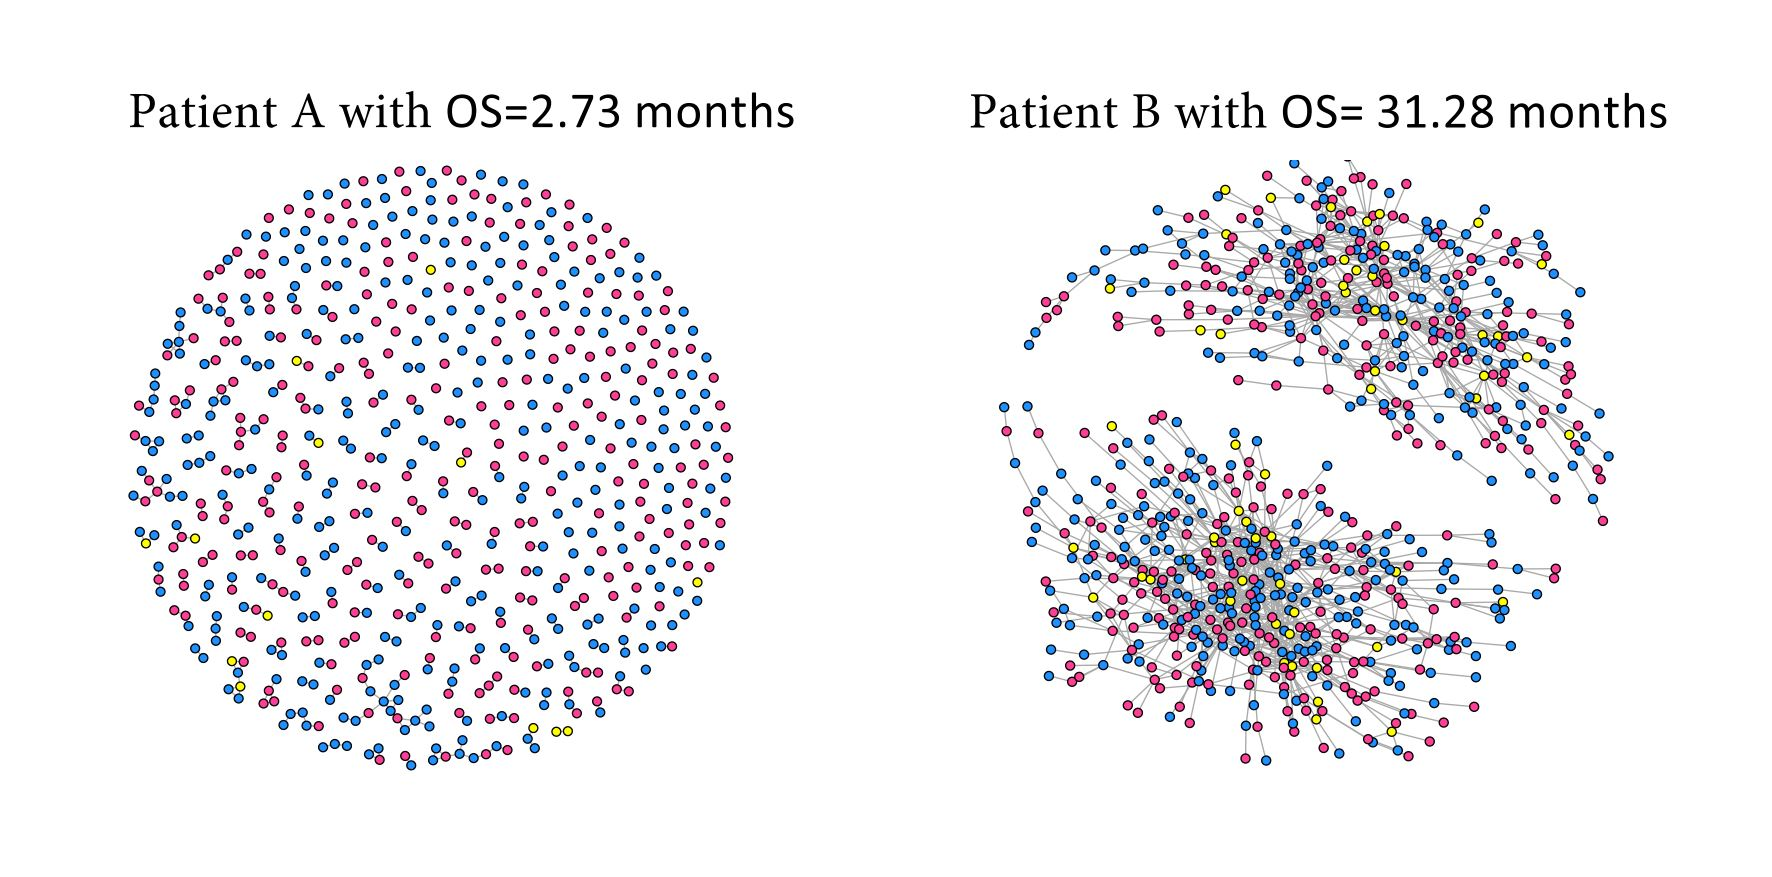
\includegraphics[scale=0.65]{TCR_ntwrk_difference.jpg}
\caption{ Network figures for two representative patients}%
{The above figure represents the TCR network diversity of two patients who participated in the drug trial. The network structures of the two patients are indicative of the differences in network complexity with respect to the $OS\_mon$ values.}
\label{fig:patient_ntwrk}
\end{figure}

\section{Real Data Analysis}\label{sec:real_data_analysis}
\subsection{Group Lasso\_CV and Group Plasso}\label{subsec:grp_cv_plasso}
The technique of Group Lasso is applied to the aggregated data with the objective to prioritize the network properties. This requires the network features to be grouped based on some underlying common factors. In our case, we aggregated those network features together that are derived from a single network property. Referring to \autoref{tab:ntwrk_features}, a total of 15 groups are created for the 15 TCR properties. The summary statistics (network features) are aggregated based on the network properties from which they were derived and then are consolidated to form feature blocks. The set of 15 feature blocks are used to build the Group Lasso models.\par
Prior to fitting the real data to the Group Lasso model, we use Cross-Validation (CV) technique to find the optimal value for the tuning parameter $\lambda$. The cross-validated technique generates two $\lambda$ values --- $\lambda_{min}$: $\lambda$ value corresponding to the minimum mean cross-validated error; $\lambda_{1SE}$: largest value of $\lambda$ such that error is within one standard error of the cross-validated errors of $\lambda_{min}$. Since $\lambda_{1SE}\ge \lambda_{min}$, the model using $\lambda_{1SE}$ has higher test error but smaller model than the model built using $\lambda_{min}$. In this study $\lambda_{1SE}=\lambda_{min}$. Using $\lambda_{min}$ value as the tuning parameter for the Group Lasso model, the prominent network properties are identified. Based on the observed data for the 65 subjects, the group indexes - 1, 5, 6 are selected as the significant properties. Note that each of these group indexes represent a unique feature block. Refer \autoref{tab:ntwrk_features}. The groups - 1, 5, 6 correspond to the \lq Membership', \lq Count\_PRE\_INFUSION' and \lq Count\_DOSE\_2' TCR network properties. The Group Lasso model with tuning parameters derived using the cross-validation technique is referred to as the \lq Group Lasso\_CV' model.
Similarly, the Group Lasso model which uses the permutation assisted tuning for finding the optimal tuning parameter is referred to as the \lq Group Plasso' model.\par
The real data is then used to feed the Group Plasso model. The original predictor variables compete with pseudo-variables (permutation copy) to determine the significant active predictors. The results from this technique is stabilized by using 10 different permutations iteratively, and evaluating the frequencies of the selected variables across those iterations. The output gives us Group - 1, 5 as the significant properties. These groups correspond to \lq Membership', \lq Count\_PRE\_INFUSION' TCR network properties.\par
We observe overlap in the TCR properties selected using Group Lasso\_CV and Group Plasso. The common groups indexes are - 1 and 5.
\subsection{Lasso\_CV and Plasso}\label{subsec:plasso_cv}
To identify the top network features the Lasso variable selection model is used on the ungrouped set of data that consists of 89 summary statistics. Lasso using cross-validation technique will be referred to as the \lq Lasso\_CV' model and the one using the permutation assisted tuning will be referred to as the \lq Plasso' model.\par
Like the technique discussed in the previous Group Lasso models, first, Cross-Validation (CV) approach is used to find the optimal value for the tuning parameter $\lambda$. Using $\lambda_{min}$ value as the tuning parameter, the Lasso\_CV model extracts the top network features significant in distinguishing between the two cohorts (\lq longer overall survival' and \lq shorter overall survival'). Feature indexes - 25, 43, 82, 89 (refer \autoref{tab:ntwrk_features}) are rendered as the top features. These feature indexes correspond to the summary statistic of the Maximum values of the TCR properties \lq Count\_PRE\_INFUSION',
\lq diam\_length', \lq eigen\_centrality', \lq centr\_eigen'. The real data is then fed into the Plasso model which identifies the top features across 10 iterations using different permutation copies.\par
Both Lasso\_CV and Plasso models generated the exact same set of features as the most significant ones.
\subsection{Exclusive Lasso\_CV}\label{subsec:exclusvlasso_cv}
Subsequently, Exclusive Lasso model is used to identify the top features from each of the network feature blocks. When using this model, the aggregated summary statistics, 15 feature blocks are used as the explanatory variables. The results from the Exclusive Lasso model should be able to reaffirm the network features selected using Lasso\_CV and Plasso models from their respective feature blocks. That is the output from the Lasso\_CV and Plasso models should be a subset of the output from the Exclusive Lasso model.\par
An optimal value of the tuning parameter $\lambda=\lambda_{1SE}$ for exclusive lasso is derived using the cross-validation approach. Similar to the group lasso model, the real data is grouped (refer \autoref{tab:ntwrk_features}). The exclusive lasso model selects the most influential features from each of the true feature blocks. It is observed that the network features selected using the Lasso\_CV and Plasso models are also selected using the Exclusive Lasso.\par
Note that permutation assisted tuning method does not work for exclusive lasso, since the model bounded by its nature will always choose at least a single feature from every feature block. As a result, exclusive lasso is unable to differentiate between the true and the pseudo-variable groups, therefore fails to perform feature selection using permutation copies.



